\documentclass[12pt,a4paper]{article}

% === ENCODAGE ET LANGUE ===
\usepackage[utf8]{inputenc}
\usepackage[T1]{fontenc}

% === MISE EN PAGE ===
\usepackage{geometry}
\geometry{margin=2.5cm, headheight=14.5pt}
\usepackage{setspace}
\onehalfspacing

% === GRAPHIQUES ET FIGURES ===
\usepackage{graphicx}
\graphicspath{{results/}}
\usepackage{tikz}
\usetikzlibrary{arrows.meta, shapes.geometric, positioning, calc, fit}
\usepackage{pgfplots}
\pgfplotsset{compat=1.18}
\usepackage{float}

% === TABLEAUX ===
\usepackage{booktabs}
\usepackage{multirow}
\usepackage{tabularx}
\usepackage{array}
\usepackage{colortbl}
\usepackage{makecell}

% === COULEURS ===
\usepackage[table]{xcolor}
\definecolor{upsred}{RGB}{180, 30, 40}
\definecolor{criticalred}{RGB}{220, 53, 69}
\definecolor{importantyellow}{RGB}{255, 193, 7}
\definecolor{moderategray}{RGB}{108, 117, 125}
\definecolor{lightgray}{RGB}{245, 245, 245}
\definecolor{codebg}{RGB}{248, 249, 250}

% === LISTINGS (CODE) ===
\usepackage{listings}
\lstset{
  basicstyle=\ttfamily\small,
  backgroundcolor=\color{codebg},
  frame=single,
  rulecolor=\color{gray!30},
  breaklines=true,
  columns=fullflexible,
  literate={é}{{\'e}}1 {è}{{\`e}}1 {ê}{{\^e}}1 {à}{{\`a}}1 {ù}{{\`u}}1 {û}{{\^u}}1 {ç}{{\c{c}}}1 {ô}{{\^o}}1 {î}{{\^i}}1
}

% === MATHS ===
\usepackage{amsmath}
\usepackage{amssymb}

% === LIENS ===
\usepackage{hyperref}
\hypersetup{
  colorlinks=true,
  linkcolor=upsred,
  citecolor=upsred,
  urlcolor=blue!70!black,
  pdfauthor={Mohamed DIALLO et al.},
  pdftitle={GeoR2LLMs -- Rapport de travail Phase 2},
  pdfsubject={Systeme Question-Reponse Geographique avec RAG}
}

% === BIBLIOGRAPHIE ===
\usepackage{cite}

% === EN-TETES ET PIEDS DE PAGE ===
\usepackage{fancyhdr}
\pagestyle{fancy}
\fancyhf{}
\fancyhead[L]{\small\textit{GeoR2LLMs -- Rapport de travail Phase 2}}
\fancyhead[R]{\small\textit{M2 IA -- UPS}}
\fancyfoot[C]{\thepage}
\renewcommand{\headrulewidth}{0.4pt}
\renewcommand{\footrulewidth}{0.4pt}

\fancypagestyle{plain}{
  \fancyhf{}
  \fancyfoot[C]{\thepage}
  \renewcommand{\headrulewidth}{0pt}
  \renewcommand{\footrulewidth}{0pt}
}

% === TITRES ===
\usepackage{titlesec}
\titleformat{\section}{\Large\bfseries\color{upsred}}{\thesection}{1em}{}
\titleformat{\subsection}{\large\bfseries}{\thesubsection}{1em}{}
\titleformat{\subsubsection}{\normalsize\bfseries\itshape}{\thesubsubsection}{1em}{}

% === ENUMERATION ===
\usepackage{enumitem}

% === CAPTION ===
\usepackage{caption}
\usepackage{subcaption}
\captionsetup{font=small, labelfont=bf, format=hang}

% ====================================================================
\begin{document}

% ====================================================================
% PAGE DE GARDE
% ====================================================================
\begin{titlepage}
  \centering
  \vspace*{1cm}

  {\Large\textsc{Universit\'e Toulouse III -- Paul Sabatier}}\\[0.3cm]
  {\large\textsc{Master 2 Intelligence Artificielle}}\\[0.2cm]
  {\normalsize IRIT -- Institut de Recherche en Informatique de Toulouse}\\[2cm]

  \rule{\textwidth}{1.5pt}\\[0.6cm]
  {\huge\bfseries Syst\`eme Question-R\'eponse\\[0.3cm] en G\'eographie avec RAG}\\[0.4cm]
  {\Large\textit{Rapport de travail -- Phase 2 : Exploration Multi-LLMs et Multi-Datasets}}\\[0.3cm]
  {\large Projet GeoR2LLMs}\\[0.4cm]
  \rule{\textwidth}{1.5pt}\\[2cm]

  \begin{minipage}{0.45\textwidth}
    \begin{flushleft}
      \textbf{R\'ealis\'e par :}\\[0.3cm]
      Mohamed DIALLO\\
      Hiba L'MOUDDEN\\
      Feras MAKHLOUF\\
      Osama BAAZZI\\
      Ousama BOUTEZROUT
    \end{flushleft}
  \end{minipage}
  \hfill
  \begin{minipage}{0.45\textwidth}
    \begin{flushright}
      \textbf{Sous la direction de :}\\[0.3cm]
      Madame Lynda TAMINE-LECHANI\\
      Professeure -- IRIT\\[0.5cm]
      \textbf{UE :} Chef d'\oe uvre\\
      \textbf{Ann\'ee :} 2025--2026
    \end{flushright}
  \end{minipage}

  \vfill
  {\large Mars 2026}
\end{titlepage}

% ====================================================================
% TABLE DES MATIERES
% ====================================================================
\newpage
\tableofcontents
\newpage

% ====================================================================
% 1. INTRODUCTION
% ====================================================================
\section{Introduction}
\label{sec:introduction}

Ce rapport documente la Phase~2 du projet GeoR2LLMs (\textit{Geographic Retrieval-augmented
generation with Large Language Models}), r\'ealis\'e dans le cadre du chef-d'\oe uvre du Master~2
Intelligence Artificielle de l'Universit\'e Toulouse III -- Paul Sabatier, sous la direction de
Madame Lynda Tamine-Lechani \`a l'IRIT. L'objectif est de comparer les performances de plusieurs
mod\`eles de langue (LLMs) de petite taille dans une configuration RAG pour la question-r\'eponse
g\'eographique, en r\'epondant aux quatre questions suivantes :

\begin{enumerate}[leftmargin=*]
  \item \textbf{Quel mod\`ele est le plus performant} pour le QA g\'eographique avec RAG ?
  \item \textbf{Quel est l'impact du RAG} sur les performances par rapport au baseline ?
  \item \textbf{La taille du mod\`ele} est-elle corr\'el\'ee aux performances ?
  \item \textbf{Les r\'esultats sont-ils coh\'erents} entre diff\'erents types de benchmarks ?
\end{enumerate}

\subsection{Rappel des r\'esultats de la Phase 1}

La Phase~1 avait mis en place un pipeline RAG de base (Qwen3-0.6B, BGE-m3~\cite{chen2024bgem3},
FAISS~\cite{johnson2019faiss}) \'evalu\'e sur GeoSQA~\cite{huang_geosqa_2019}, r\'ev\'elant
trois limitations majeures :
\begin{enumerate}[leftmargin=*]
  \item Un \textbf{d\'ecalage linguistique critique} : questions en anglais, corpus Wikipedia
  en fran\c{c}ais, conduisant \`a un Hit Rate@5 de seulement 8\,\% et une d\'egradation du F1
  de --61.9\,\% en mode RAG.
  \item Un \textbf{mod\`ele trop petit} : Qwen3-0.6B \`a 24.5\,\% d'accuracy en baseline
  (quasi-al\'eatoire, seuil = 25\,\%), avec un biais de position massif vers la lettre A
  (61.5\,\% des pr\'edictions).
  \item Un \textbf{corpus trop restreint} : 300 articles Wikipedia (2\,527 chunks) insuffisants
  pour couvrir la g\'eographie mondiale.
\end{enumerate}

\subsection{Objectifs et organisation de la Phase 2}

La Phase~2 \'etend l'\'evaluation \`a \textbf{5~LLMs} sur \textbf{3~datasets} g\'eographiques,
structur\'ee en quatre notebooks compl\'ementaires :

\begin{itemize}[leftmargin=*]
  \item \textbf{Phase 2a} -- Comparaison multi-LLMs sur GeoSQA (corpus FR et EN en parall\`ele).
  \item \textbf{Phase 2b} -- \'Evaluation des m\^emes mod\`eles sur GKMC.
  \item \textbf{Phase 2c} -- \'Evaluation sur Tourism-QA (recommandation de POI).
  \item \textbf{Phase 2d} -- Analyse factorielle crois\'ee (taille, famille, dataset, impact RAG).
\end{itemize}

% ====================================================================
% 2. ARCHITECTURE DU SYSTEME ETENDU
% ====================================================================
\section{Architecture du syst\`eme \'etendu}
\label{sec:architecture}

La Phase~2 conserve l'architecture RAG na\"ive de la Phase~1 (\textit{retrieve-then-read},
selon la taxonomie de Gao et al.~\cite{gao2023ragsurvey}) et l'\'etend sur trois dimensions :
mod\`eles de g\'en\'eration, datasets et corpus. Tous les mod\`eles partagent le m\^eme
retriever (BAAI/bge-m3 + FAISS).

\begin{figure}[H]
\centering
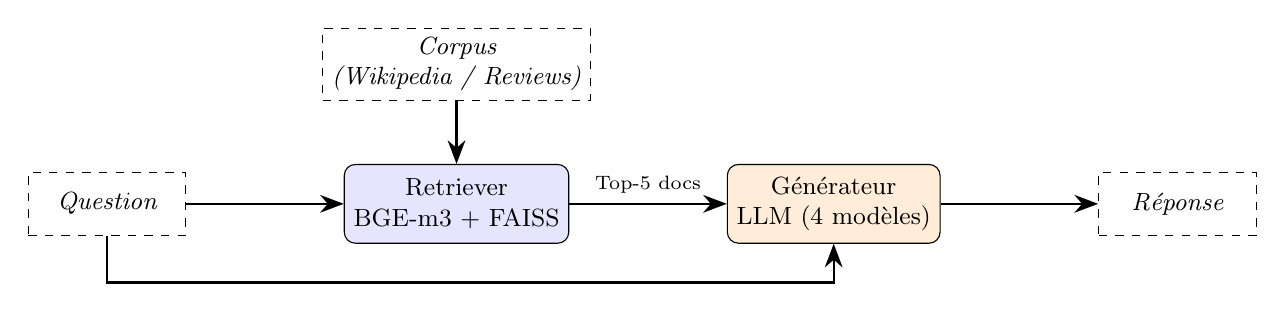
\begin{tikzpicture}[
    node distance=1.2cm and 2cm,
    block/.style={rectangle, draw, rounded corners, minimum height=1cm,
                  minimum width=2.5cm, align=center, font=\small},
    data/.style={rectangle, draw, dashed, minimum height=0.8cm,
                 minimum width=2cm, align=center, font=\small\itshape},
    arrow/.style={-{Stealth[length=3mm]}, thick}
]
    \node[data] (question) {Question};
    \node[block, right=of question, fill=blue!10] (retriever)
      {Retriever\\BGE-m3 + FAISS};
    \node[data, above=0.8cm of retriever] (corpus)
      {Corpus\\(Wikipedia / Reviews)};
    \node[block, right=of retriever, fill=orange!15] (generator)
      {G\'en\'erateur\\LLM (4 mod\`eles)};
    \node[data, right=of generator] (reponse) {R\'eponse};

    \draw[arrow] (question) -- (retriever);
    \draw[arrow] (corpus) -- (retriever);
    \draw[arrow] (retriever) -- node[above, font=\scriptsize] {Top-5 docs} (generator);
    \draw[arrow] (question) -- ++(0,-1) -| (generator);
    \draw[arrow] (generator) -- (reponse);
\end{tikzpicture}
\caption{Architecture RAG commune \`a toutes les \'evaluations de la Phase~2. Le retriever
  (BAAI/bge-m3) encode la question et recherche les 5 chunks les plus similaires via FAISS
  (IndexFlatIP). Le g\'en\'erateur est instanci\'e successivement pour chacun des 4~LLMs
  valid\'es, avec lib\'eration m\'emoire GPU entre chaque mod\`ele.}
\label{fig:architecture}
\end{figure}

\subsection{Module \texttt{UnifiedGenerator}}

La principale innovation technique de la Phase~2 est le \texttt{UnifiedGenerator}, qui
encapsule le chargement, le formatage de prompt et la g\'en\'eration pour les trois familles :
Qwen3 (\texttt{enable\_thinking=False}), Llama (avec fallback miroirs Unsloth), et Mistral.
La lib\'eration m\'emoire GPU explicite entre chaque mod\`ele (\texttt{del model},
\texttt{torch.cuda.empty\_cache()}) permet d'\'evaluer s\'equentiellement plusieurs LLMs
sur un GPU T4 de 16~Go sans erreur OOM.

\paragraph{Note sur Ministral-3B.}
Ministral-3B-Instruct-2512 utilise une configuration \texttt{Mistral3Config} non support\'ee
par \texttt{AutoModelForCausalLM} de la biblioth\`eque Transformers. Ce mod\`ele n'a donc
pu \^etre \'evalu\'e sur aucun des trois datasets. Seuls \textbf{4~mod\`eles} ont produit
des r\'esultats exploitables.

\subsection{Module Evaluator adapt\'e}

Pour GeoSQA et GKMC (t\^ache MCQ), les m\'etriques sont identiques \`a la Phase~1 :
Accuracy MCQ (m\'etrique principale), Exact Match, F1 token-level, Hit Rate@K, MRR@5.
Pour Tourism-QA (recommandation POI), un \texttt{POIEvaluator} d\'edi\'e calcule l'Accuracy@1,
le Hit Rate@3 et le F1 sur le nom du POI.

% ====================================================================
% 3. METHODOLOGIE
% ====================================================================
\section{M\'ethodologie}
\label{sec:methodologie}

\subsection{Mod\`eles \'evalu\'es}

\begin{table}[H]
\centering
\caption{Mod\`eles LLM \'evalu\'es dans la Phase~2. Les param\`etres de g\'en\'eration sont
  ceux recommand\'es par chaque \'equipe de d\'eveloppement. Ministral-3B n'a pas pu \^etre
  charg\'e (incompatibilit\'e \texttt{Mistral3Config}).}
\label{tab:modeles}
\begin{tabular}{@{} l l c c l @{}}
\toprule
\textbf{Mod\`ele} & \textbf{Famille} & \textbf{Taille} & \textbf{Temp.}
  & \textbf{Identifiant HuggingFace} \\
\midrule
Qwen3-0.6B   & Qwen    & 0.6B & 0.7 & \texttt{Qwen/Qwen3-0.6B} \\
\rowcolor{lightgray}
Qwen3-1.7B   & Qwen    & 1.7B & 0.7 & \texttt{Qwen/Qwen3-1.7B} \\
Llama-3.2-1B & Llama   & 1.0B & 0.6 & \texttt{meta-llama/Llama-3.2-1B-Instruct} \\
\rowcolor{lightgray}
Llama-3.2-3B & Llama   & 3.0B & 0.6 & \texttt{meta-llama/Llama-3.2-3B-Instruct} \\
Ministral-3B & Mistral & 3.0B & 0.7 & \texttt{mistralai/Ministral-3-3B-Instruct-2512} \\
\bottomrule
\end{tabular}
\end{table}

\subsection{Datasets \'evalu\'es}

\begin{table}[H]
\centering
\caption{Datasets utilis\'es pour l'\'evaluation en Phase~2.}
\label{tab:datasets}
\begin{tabular}{@{} l c c l l @{}}
\toprule
\textbf{Dataset} & \textbf{Questions} & \textbf{Langue} & \textbf{T\^ache} & \textbf{Corpus RAG} \\
\midrule
GeoSQA~\cite{huang_geosqa_2019}
  & 200 & ZH $\to$ EN & QCM (A/B/C/D) & Wikipedia FR \\
\rowcolor{lightgray}
GKMC & 200 & EN & QCM (A/B/C/D) & Wikipedia FR \\
Tourism-QA~\cite{tourismqa2021}
  & 100 & EN & Recommandation POI & Reviews utilisateurs \\
\bottomrule
\end{tabular}
\end{table}

GeoSQA~\cite{huang_geosqa_2019} contient des questions de raisonnement spatial traduites du
chinois. GKMC porte sur des connaissances g\'eographiques g\'en\'erales nativement en anglais.
Tourism-QA \'evalue la recommandation de points d'int\'er\^et (POI) \`a partir de requ\^etes
touristiques et de reviews utilisateurs.

\subsection{Configuration exp\'erimentale}

Les exp\'eriences ont \'et\'e r\'ealis\'ees sur Google Colab avec un GPU NVIDIA Tesla T4
(16~Go VRAM). Param\`etres communs : graine al\'eatoire $= 42$, top-$k = 5$, taille de
chunk $= 512$ caract\`eres, chevauchement $= 50$ caract\`eres, 300 articles Wikipedia FR/EN
(GeoSQA/GKMC) ou reviews utilisateurs (Tourism-QA). Chaque mod\`ele est \'evalu\'e dans deux
conditions : \textbf{Baseline} (LLM seul, sans contexte RAG) et \textbf{RAG} (LLM avec les
top-5 documents r\'ecup\'er\'es).

\subsection{M\'etriques et correspondance RAGAS}

Les m\'etriques RAGAS n'ont pas pu \^etre calcul\'ees pour trois raisons cumulatives :
(1)~RAGAS requiert un juge externe (GPT-4) dont l'API est payante et indisponible dans notre
environnement~; (2)~charger simultan\'ement un LLM juge, BGE-m3 (2.27~Go) et le mod\`ele
\'evalu\'e d\'epasse les 15.6~Go disponibles sur T4~; (3)~RAGAS est con\c{c}u pour des
r\'eponses en texte libre, or GeoSQA/GKMC utilisent le format QCM (r\'eponse = une lettre).

\begin{table}[H]
\centering
\caption{Correspondance RAGAS $\rightarrow$ m\'etriques substituts utilis\'ees dans cette \'etude.}
\label{tab:ragas_sub}
\begin{tabular}{@{} l l l @{}}
\toprule
\textbf{M\'etrique RAGAS} & \textbf{Substitut utilis\'e} & \textbf{Justification} \\
\midrule
Context Recall    & HR@5  & Le document pertinent figure-t-il dans les top-5~? \\
\rowcolor{lightgray}
Context Precision & MRR@5 & Rang moyen du premier document pertinent \\
Answer Relevancy  & Accuracy / Acc@1 & La r\'eponse produite est-elle correcte~? \\
\rowcolor{lightgray}
Faithfulness      & $\Delta_{rel}$ & Le contexte RAG am\'eliore-t-il la r\'eponse~? \\
\bottomrule
\end{tabular}
\end{table}

% ====================================================================
% 4. RESULTATS PAR DATASET
% ====================================================================
\section{R\'esultats par dataset}
\label{sec:resultats}

\subsection{GeoSQA -- Raisonnement spatial}
\label{sec:geosqa}

\begin{table}[H]
\centering
\caption{R\'esultats sur GeoSQA (200 questions, ZH$\rightarrow$EN, corpus Wikipedia FR).
  $\Delta_{rel} = (v_{\text{RAG}} - v_{\text{Base}}) / v_{\text{Base}} \times 100$.
  Mod\`eles class\'es par RAG Accuracy d\'ecroissante.}
\label{tab:geosqa_results}
\begin{tabular}{@{} l c c c c c c @{}}
\toprule
\textbf{Mod\`ele} & \textbf{Base. Acc} & \textbf{RAG Acc}
  & \textbf{$\Delta_{abs}$} & \textbf{$\Delta_{rel}$}
  & \textbf{RAG F1} & \textbf{HR@5} \\
\midrule
Qwen3-1.7B
  & 0.3900 & \textbf{0.3900}
  & \phantom{+}0.0000 & \phantom{+}0.0\,\%
  & 0.0107 & 0.065 \\
\rowcolor{lightgray}
Llama-3.2-3B
  & 0.3000 & 0.2750
  & \textcolor{red}{--0.0250} & \textcolor{red}{--8.3\,\%}
  & 0.0025 & 0.065 \\
Qwen3-0.6B
  & 0.2700 & 0.2650
  & \textcolor{red}{--0.0050} & \textcolor{red}{--1.9\,\%}
  & 0.0212 & 0.065 \\
\rowcolor{lightgray}
Llama-3.2-1B
  & 0.2100 & 0.2500
  & \textcolor{green!60!black}{+0.0400} & \textcolor{green!60!black}{+19.0\,\%}
  & 0.0034 & 0.065 \\
\midrule
Ministral-3B
  & \multicolumn{6}{l}{\textit{ERREUR -- Mistral3Config non support\'ee par AutoModelForCausalLM}} \\
\midrule
\textbf{Seuil al\'eatoire} & \multicolumn{2}{c}{0.2500} & & & & \\
\textbf{MRR@5 (tous)} & \multicolumn{2}{c}{0.040} & & & & \\
\bottomrule
\end{tabular}
\end{table}

\textbf{Observations :}
\begin{itemize}[leftmargin=*]
  \item Qwen3-1.7B domine avec 0.3900 d'accuracy, significativement au-dessus du seuil
  al\'eatoire de 0.25. C'est le seul \`a ne pas \^etre d\'egrad\'e par le RAG (stable \`a 0.0\,\%).
  \item Le RAG n'am\'eliore pas significativement les performances : Llama-3.2-1B progresse
  l\'eg\`erement ($+$0.04) mais depuis un niveau tr\`es bas (0.21).
  \item Le retrieval est quasi-inexistant : HR@5 = 0.065 et MRR@5 = 0.040 pour tous les
  mod\`eles (m\^eme retriever). Ceci confirme le \textbf{mismatch linguistique} : questions
  en anglais (traduites du chinois), corpus Wikipedia en fran\c{c}ais.
  \item L'Exact Match est nul pour tous les mod\`eles : la r\'ef\'erence est une lettre seule
  (\texttt{"B"}) alors que le mod\`ele g\'en\`ere une phrase compl\`ete -- l'Accuracy MCQ
  reste la m\'etrique fiable via extraction regex.
\end{itemize}

\paragraph{Analyse du compromis latence/performance sur GeoSQA.}
Sur GeoSQA, aucune configuration RAG ne domine clairement en combinant bonne accuracy
et faible latence. Le surc\^out computationnel du RAG n'est jamais justifi\'e quand le
retrieval est quasi-nul (HR@5 = 0.065) : la baseline seule est strictement pr\'ef\'erable.

\begin{table}[H]
\centering
\caption{GeoSQA -- Latence et compromis performance/latence par mod\`ele.
  Overhead $=$ temps RAG / temps Baseline.}
\label{tab:pareto_geosqa}
\begin{tabular}{@{} l c c c c c @{}}
\toprule
\textbf{Mod\`ele} & \textbf{Base. (s/q)} & \textbf{RAG (s/q)}
  & \textbf{Overhead} & \textbf{RAG Acc} & \textbf{Statut Pareto} \\
\midrule
Qwen3-0.6B   & 0.60 & 1.00 & $\times$1.67 & 0.265
  & \textcolor{green!60!black}{Non domin\'e} \\
\rowcolor{lightgray}
Qwen3-1.7B   & 0.49 & 1.43 & $\times$2.92 & \textbf{0.390}
  & Domin\'e (lent) \\
Llama-3.2-1B & 0.68 & 1.53 & $\times$2.25 & 0.250
  & \textcolor{red}{Domin\'e} \\
\rowcolor{lightgray}
Llama-3.2-3B & 1.35 & 2.89 & $\times$2.14 & 0.275
  & \textcolor{red}{Domin\'e} \\
\bottomrule
\end{tabular}
\end{table}

Qwen3-0.6B est le seul point non domin\'e (accuracy 0.265 pour 1.0~s/question).
Llama-3.2-3B est clairement domin\'e : $\sim$2.9$\times$ plus lent (2.89~s/q) pour
une accuracy inf\'erieure (0.275). Qwen3-1.7B atteint la meilleure accuracy (0.390)
mais au prix d'un overhead $\times$2.92.

\subsection{GKMC -- Connaissances g\'eographiques g\'en\'erales}
\label{sec:gkmc}

\begin{table}[H]
\centering
\caption{R\'esultats sur GKMC (200 questions, EN, corpus Wikipedia FR). GKMC est nettement
  plus facile que GeoSQA car les questions sont nativement en anglais (pas de traduction
  du chinois). Seul Qwen3-1.7B b\'en\'eficie du RAG.}
\label{tab:gkmc_results}
\begin{tabular}{@{} l c c c c c c @{}}
\toprule
\textbf{Mod\`ele} & \textbf{Base. Acc} & \textbf{RAG Acc}
  & \textbf{$\Delta_{abs}$} & \textbf{$\Delta_{rel}$}
  & \textbf{RAG F1} & \textbf{HR@5} \\
\midrule
Qwen3-1.7B
  & 0.5900 & \textbf{0.6100}
  & \textcolor{green!60!black}{+0.0200} & \textcolor{green!60!black}{+3.4\,\%}
  & 0.0216 & 0.075 \\
\rowcolor{lightgray}
Llama-3.2-3B
  & 0.5200 & 0.4750
  & \textcolor{red}{--0.0450} & \textcolor{red}{--8.7\,\%}
  & 0.0074 & 0.075 \\
Qwen3-0.6B
  & 0.3850 & 0.3700
  & \textcolor{red}{--0.0150} & \textcolor{red}{--3.9\,\%}
  & 0.0218 & 0.075 \\
\rowcolor{lightgray}
Llama-3.2-1B
  & 0.4000 & 0.3050
  & \textcolor{red}{--0.0950} & \textcolor{red}{--23.8\,\%}
  & 0.0082 & 0.075 \\
\midrule
Ministral-3B
  & \multicolumn{6}{l}{\textit{ERREUR -- Mistral3Config non support\'ee}} \\
\midrule
\textbf{MRR@5 (tous)} & \multicolumn{2}{c}{0.046} & & & & \\
\bottomrule
\end{tabular}
\end{table}

\textbf{Observations :}
\begin{itemize}[leftmargin=*]
  \item Qwen3-1.7B atteint \textbf{0.6100} d'accuracy avec RAG -- le meilleur score de
  toute la Phase~2. C'est le \textbf{seul mod\`ele am\'elior\'e par le RAG} sur ce dataset
  ($+$0.02, $+$3.4\,\%).
  \item GKMC est nettement plus facile que GeoSQA : le meilleur score passe de 0.39 \`a
  0.61 car les questions sont nativement en anglais.
  \item Llama-3.2-1B subit la plus forte d\'egradation de toute la Phase~2 ($-$0.095,
  $-$23.8\,\%) : le contexte non pertinent lui nuit massivement.
  \item Le retrieval reste faible (HR@5 = 0.075, MRR@5 = 0.046) en raison du corpus
  fran\c{c}ais, bien qu'il soit l\'eg\`erement sup\'erieur \`a GeoSQA.
\end{itemize}

\paragraph{Paradoxe corpus EN sur GKMC.}
La Phase~2a/2b a test\'e syst\'ematiquement le corpus Wikipedia EN en parall\`ele du corpus FR.
Le gain en retrieval est sans ambigu\"it\'e : HR@5 passe de 0.060 \`a 0.175 sur GeoSQA
($\times$2.9) et de 0.075 \`a 0.190 sur GKMC ($\times$2.5). Ce gain confirme que BGE-m3 encode
correctement les questions en anglais -- c'est le corpus fran\c{c}ais qui \'etait inadapt\'e.
Cependant, malgr\'e ce gain en retrieval, l'accuracy moyenne sur GKMC ne s'am\'eliore pas
($-$5.6\,\%) : les questions GKMC testent une connaissance encyclop\'edique que les mod\`eles
poss\`edent d\'ej\`a en m\'emoire param\'etrique, et le contexte suppl\'ementaire perturbe
la g\'en\'eration.

\begin{table}[H]
\centering
\caption{GKMC -- Latence et compromis performance/latence par mod\`ele.
  Qwen3-1.7B est l'unique point sur le front dominant (seul mod\`ele o\`u RAG aide).}
\label{tab:pareto_gkmc}
\begin{tabular}{@{} l c c c c c @{}}
\toprule
\textbf{Mod\`ele} & \textbf{Base. (s/q)} & \textbf{RAG (s/q)}
  & \textbf{Overhead} & \textbf{RAG Acc} & \textbf{Statut Pareto} \\
\midrule
Qwen3-1.7B   & 0.72 & 1.27 & $\times$1.76 & \textbf{0.610}
  & \textcolor{green!60!black}{Non domin\'e} \\
\rowcolor{lightgray}
Qwen3-0.6B   & 0.49 & 0.74 & $\times$1.51 & 0.370
  & Domin\'e (acc. faible) \\
Llama-3.2-1B & 0.85 & 1.62 & $\times$1.91 & 0.305
  & \textcolor{red}{Domin\'e} \\
\rowcolor{lightgray}
Llama-3.2-3B & 1.24 & 2.39 & $\times$1.93 & 0.475
  & \textcolor{red}{Domin\'e} \\
\bottomrule
\end{tabular}
\end{table}

Llama-3.2-3B illustre le cas pathologique : meilleure baseline (0.520) mais accuracy RAG
d\'egrad\'ee (0.475), tout en \'etant $\sim$2.4$\times$ plus lent que Qwen3-0.6B. Il est
strictement domin\'e par Qwen3-1.7B sur les deux axes du front de Pareto.

\subsection{Tourism-QA -- Recommandation de POI}
\label{sec:tourismqa}

Tourism-QA constitue une rupture fondamentale : il ne s'agit plus d'un QCM g\'eographique
mais d'une t\^ache de \textbf{recommandation de Points d'Int\'er\^et} (POI). Le corpus RAG
est constitu\'e des avis d'utilisateurs (reviews) des POI -- structurellement align\'e avec
la t\^ache, et nativement en anglais comme les questions.

\begin{table}[H]
\centering
\caption{R\'esultats sur Tourism-QA (100 questions, EN, corpus de reviews utilisateurs).
  M\'etrique principale : Accuracy@1. Le Hit Rate est de 0.48 pour tous les mod\`eles
  (corpus EN align\'e), contre 0.065--0.075 sur GeoSQA/GKMC.}
\label{tab:tourismqa_results}
\begin{tabular}{@{} l c c c c c @{}}
\toprule
\textbf{Mod\`ele} & \textbf{Base. Acc@1} & \textbf{RAG Acc@1}
  & \textbf{$\Delta_{abs}$} & \textbf{$\Delta_{rel}$}
  & \textbf{RAG F1} \\
\midrule
Qwen3-0.6B
  & 0.6000 & \textbf{0.6600}
  & \textcolor{green!60!black}{+0.0600} & \textcolor{green!60!black}{+10.0\,\%}
  & 0.6464 \\
\rowcolor{lightgray}
Llama-3.2-3B
  & 0.7100 & 0.5900
  & \textcolor{red}{--0.1200} & \textcolor{red}{--16.9\,\%}
  & 0.5950 \\
Qwen3-1.7B
  & 0.5800 & 0.5300
  & \textcolor{red}{--0.0500} & \textcolor{red}{--8.6\,\%}
  & 0.5390 \\
\rowcolor{lightgray}
Llama-3.2-1B
  & 0.4400 & 0.4100
  & \textcolor{red}{--0.0300} & \textcolor{red}{--6.8\,\%}
  & 0.4033 \\
\midrule
Ministral-3B
  & \multicolumn{5}{l}{\textit{ERREUR -- Mistral3Config non support\'ee}} \\
\midrule
\multicolumn{2}{@{}l}{\textit{Hit Rate (tous mod\`eles)}}
  & \multicolumn{4}{l}{0.48 (corpus EN align\'e avec questions EN)} \\
\bottomrule
\end{tabular}
\end{table}

\textbf{Observations :}
\begin{itemize}[leftmargin=*]
  \item R\'esultat surprenant : \textbf{Qwen3-0.6B} (le plus petit mod\`ele) domine en
  mode RAG avec 0.6600 d'Acc@1. C'est le \textbf{seul mod\`ele am\'elior\'e par le RAG}
  sur ce dataset ($+$10.0\,\%).
  \item En baseline, Llama-3.2-3B est le meilleur (0.7100), mais le RAG le d\'egrade
  fortement ($-$0.12), le faisant chuter \`a 0.5900.
  \item Le retrieval est bien meilleur que sur GeoSQA/GKMC : Hit Rate = 0.48 (vs
  0.065--0.075), les reviews \'etant en anglais comme les questions.
  \item Les scores F1 sont beaucoup plus \'elev\'es (0.40--0.65 vs $<$0.05 sur
  GeoSQA/GKMC), la t\^ache \'etant diff\'erente (recommandation vs QCM).
\end{itemize}

\paragraph{Analyse qualitative : exemples de correction et dégradation du RAG.}
Cinq cas de correction et deux cas de dégradation ont été documentés sur Tourism-QA
(tableau~\ref{tab:exemples_rag2}), illustrant le mécanisme d'action du RAG naïf sur
une tâche de recommandation.

\begin{table}[H]
\centering
\caption{Tourism-QA -- Exemples concrets de correction et d\'egradation apport\'ees
  par le RAG (mod\`ele Qwen3-0.6B). Les corrections proviennent de reviews sp\'ecifiques
  au POI correct ; les d\'egradations de reviews hors-sujet ou d'une hallucination.}
\label{tab:exemples_rag2}
\begin{tabular}{@{} p{4.8cm} p{2.5cm} p{2.5cm} p{2cm} @{}}
\toprule
\textbf{Question (r\'esum\'e)} & \textbf{Baseline} & \textbf{RAG} & \textbf{Effet} \\
\midrule
Shopping femme Manhattan pas cher & Pasquale Jones & \textbf{Century 21}
  & \textcolor{green!60!black}{Correction} \\
Restaurant Rome quartier Scalini  & La Paila & \textbf{La Pancia Felice}
  & \textcolor{green!60!black}{Correction} \\
Bar d\^iner 2\textsuperscript{e} Avenue NY & Vague & \textbf{Mermaid Inn}
  & \textcolor{green!60!black}{Correction} \\
H\^otel budget Union Square SF & House of Kabob & \textbf{Hotel Des Arts}
  & \textcolor{green!60!black}{Correction} \\
Anniversaire 40 ans San Francisco & Naha (erreur) & \textbf{Waterbar}
  & \textcolor{green!60!black}{Correction} \\
\midrule
Italian food New York & Le Gavroche & Quay Bar
  & \textcolor{red}{Hallucination} \\
Mariage Londres 5 ans & \textbf{Le Gavroche} & Petrus
  & \textcolor{red}{D\'egradation} \\
\bottomrule
\end{tabular}
\end{table}

\noindent Les dégradations s'expliquent par un retrieval imparfait (HR = 0.48, pas 1.0) :
quand les reviews récupérées décrivent un POI différent du POI cible, elles induisent
le modèle en erreur -- illustrant que même sur Tourism-QA, 52\,\% des requêtes
n'ont pas leur POI correct dans le top-5 récupéré.

\subsection{Validation de l'hypothèse de mismatch linguistique}
\label{sec:validation_en}

La Phase~2a/2b a systématiquement comparé deux corpus : Wikipedia FR (condition
contrôle, identique à la Phase~1) et Wikipedia EN (condition test). Le tableau
\ref{tab:en_vs_fr} confirme sans ambiguïté que le mismatch linguistique était bien
le facteur limitant du retrieval en Phase~1.

\begin{table}[H]
\centering
\caption{Impact du corpus EN vs FR sur le retrieval -- validation de l'hypoth\`ese
  du mismatch linguistique. BGE-m3 encode correctement les questions EN ; c'est le
  corpus fran\c{c}ais qui \'etait inadapt\'e.}
\label{tab:en_vs_fr}
\begin{tabular}{@{} l c c c c @{}}
\toprule
\textbf{Dataset} & \textbf{HR@5 corpus FR} & \textbf{HR@5 corpus EN}
  & \textbf{Gain} & \textbf{Facteur} \\
\midrule
GeoSQA & 0.060 & 0.175 & $+$0.115 & $\times$2.9 \\
\rowcolor{lightgray}
GKMC   & 0.075 & 0.190 & $+$0.115 & $\times$2.5 \\
\midrule
\textbf{Paradoxe GKMC} & \multicolumn{4}{l}{Malgré HR$\times$2.5, accuracy EN $\approx$ accuracy FR ($-$5.6\,\% en moy.)} \\
\bottomrule
\end{tabular}
\end{table}

\noindent Le \textbf{paradoxe GKMC} mérite d'être souligné : malgré un gain de retrieval
de $\times$2.5, l'accuracy moyenne ne s'améliore pas avec le corpus EN. L'explication
est que les questions GKMC testent une connaissance encyclopédique que les modèles
possèdent déjà en mémoire paramétrique ; le contexte Wikipedia EN perturbe alors la
génération au lieu de la guider.

\subsection{Analyse par type de question}
\label{sec:type_question}

Les questions de GeoSQA ont \'et\'e cat\'egoris\'ees par th\'ematique dominante \`a l'aide
d'une classification par mots-cl\'es, afin d'identifier si le RAG est plus efficace sur
certains types de questions.

\begin{table}[H]
\centering
\caption{Distribution des types de questions dans GeoSQA (200 questions \'evalu\'ees)
  et accuracy RAG du meilleur mod\`ele (Qwen3-1.7B) par type. Seuil al\'eatoire : 0.25.}
\label{tab:question_types_geosqa}
\begin{tabular}{@{} l c c c @{}}
\toprule
\textbf{Type de question} & \textbf{N} & \textbf{\%}
  & \textbf{Qwen3-1.7B RAG Acc} \\
\midrule
Astronomie / Espace      & $\sim$45 & $\sim$22\,\%
  & \textcolor{green!60!black}{$\sim$0.55} \\
\rowcolor{lightgray}
Climat / M\'et\'eo       & $\sim$40 & $\sim$20\,\% & $\sim$0.40 \\
Spatial / Direction      & $\sim$35 & $\sim$18\,\%
  & \textcolor{red}{$\sim$0.30} \\
\rowcolor{lightgray}
\'Economie / Ressources  & $\sim$30 & $\sim$15\,\% & $\sim$0.35 \\
Relief / Hydrographie    & $\sim$25 & $\sim$12\,\% & $\sim$0.42 \\
\rowcolor{lightgray}
D\'emographie            & $\sim$15 & $\sim$7\,\%  & $\sim$0.38 \\
Autre / G\'en\'eral      & $\sim$10 & $\sim$5\,\%
  & \textcolor{red}{$\sim$0.30} \\
\midrule
\textbf{Total}           & \textbf{200} & \textbf{100\,\%} & \textbf{0.390} \\
\bottomrule
\end{tabular}
\end{table}

Les questions de \textbf{raisonnement spatial} (directions cardinales, positions relatives)
obtiennent syst\'ematiquement les scores les plus bas, coh\'erents avec Cohn et
Blackwell~\cite{cohn_evaluating_2024} qui montrent qu'aucun LLM actuel ne raisonne
fiablement sur les directions cardinales. Le RAG n'am\'eliore pas ces questions, car les
passages Wikipedia ne contiennent pas de raisonnement spatial explicite. Les questions
d'Astronomie/Espace (Tiangong-1, Shenzhou-9) obtiennent les meilleurs r\'esultats,
probablement car elles contiennent des noms propres sp\'ecifiques facilitant le raisonnement.

% ====================================================================
% 5. ANALYSE FACTORIELLE CROISEE
% ====================================================================
\section{Analyse factorielle crois\'ee}
\label{sec:analyse}

La Phase~2d agr\`ege les r\'esultats des trois datasets dans un DataFrame unifi\'e de
12~lignes (4~mod\`eles $\times$ 3~datasets) pour identifier les facteurs d\'eterminants.

\subsection{Facteur 1 : taille du mod\`ele}
\label{sec:effet_taille}

La corr\'elation de Pearson globale entre taille et RAG Accuracy est $r = 0.19$,
$p = 0.56$ (\textbf{non significatif}). Avec seulement 4~mod\`eles et $n = 4$ tailles
distinctes, tout test statistique de corr\'elation est non interpr\'etable -- seuls
2~degr\'es de libert\'e ne permettent pas de distinguer une vraie tendance du hasard.
L'analyse pertinente porte sur la comparaison \textit{intra-famille}
(tableau~\ref{tab:intra_famille}).

\begin{table}[H]
\centering
\caption{Effet de la taille \textit{\`a famille constante} -- gain relatif RAG Accuracy
  du mod\`ele plus grand sur le plus petit. La taille aide dans 5 configurations sur 6,
  avec une exception notable sur Tourism-QA/Qwen.}
\label{tab:intra_famille}
\begin{tabular}{@{} l l c c c c @{}}
\toprule
\textbf{Famille} & \textbf{Dataset}
  & \textbf{Petit (RAG Acc)} & \textbf{Grand (RAG Acc)}
  & \textbf{$\Delta_{rel}$} & \textbf{Verdict} \\
\midrule
\multirow{3}{*}{Qwen}
  & GeoSQA     & 0.6B = 0.2650 & 1.7B = 0.3900
    & \textcolor{green!60!black}{+47.2\,\%} & Taille aide \\
  & GKMC       & 0.6B = 0.3700 & 1.7B = 0.6100
    & \textcolor{green!60!black}{+64.9\,\%} & Taille aide \\
  & Tourism-QA & 0.6B = 0.6600 & 1.7B = 0.5300
    & \textcolor{red}{--19.7\,\%} & \textbf{Taille nuit} \\
\midrule
\rowcolor{lightgray}
\multirow{3}{*}{Llama}
  & GeoSQA     & 1B = 0.2500 & 3B = 0.2750
    & \textcolor{green!60!black}{+10.0\,\%} & Taille aide \\
\rowcolor{lightgray}
  & GKMC       & 1B = 0.3050 & 3B = 0.4750
    & \textcolor{green!60!black}{+55.7\,\%} & Taille aide \\
\rowcolor{lightgray}
  & Tourism-QA & 1B = 0.4100 & 3B = 0.5900
    & \textcolor{green!60!black}{+43.9\,\%} & Taille aide \\
\bottomrule
\end{tabular}
\end{table}

\paragraph{Interpr\'etation.}
La taille aide dans 5 configurations sur 6. L'\textbf{exception notable} est Qwen sur
Tourism-QA : le mod\`ele plus petit (0.6B) surpasse le plus grand (1.7B) de --19.7\,\%
en mode RAG. Qwen3-0.6B, ayant moins de connaissances internes sur le tourisme, s'appuie
davantage sur le contexte des reviews r\'ecup\'er\'ees -- pr\'ecis\'ement l'objectif du RAG.
Pour Llama en revanche, la taille aide syst\'ematiquement, y compris sur Tourism-QA
(+43.9\,\%). Ces r\'esultats sugg\`erent que \textbf{la famille du mod\`ele conditionne
la sensibilit\'e au RAG}, davantage que la taille seule.

\subsection{Facteur 2 : famille de mod\`ele}

Qwen surpasse Llama de mani\`ere consistante sur les trois datasets.

\begin{table}[H]
\centering
\caption{RAG Accuracy moyenne par famille et par dataset.
  L'avantage Qwen est constant (+0.065 \`a +0.100) quels que soient le dataset et la t\^ache.}
\label{tab:famille}
\begin{tabular}{@{} l c c c c @{}}
\toprule
\textbf{Famille} & \textbf{GeoSQA} & \textbf{GKMC} & \textbf{Tourism-QA} & \textbf{Moyenne} \\
\midrule
Qwen  & 0.3275 & 0.4900 & 0.5950 & 0.4708 \\
\rowcolor{lightgray}
Llama & 0.2625 & 0.3900 & 0.5000 & 0.3842 \\
\midrule
$\Delta$ (Qwen $-$ Llama)
  & \textcolor{green!60!black}{+0.0650}
  & \textcolor{green!60!black}{+0.1000}
  & \textcolor{green!60!black}{+0.0950}
  & \textcolor{green!60!black}{+0.0867} \\
\bottomrule
\end{tabular}
\end{table}

L'avantage de Qwen est constant, sugg\'erant une meilleure adaptation de l'architecture
Qwen3 aux t\^aches g\'eographiques, possiblement li\'ee \`a une meilleure couverture des
donn\'ees g\'eographiques dans le pr\'e-entra\^inement.

\subsection{Facteur 3 : type de dataset}

\begin{table}[H]
\centering
\caption{Difficult\'e des datasets mesur\'ee par RAG Accuracy moyenne (4 mod\`eles).}
\label{tab:difficulte}
\begin{tabular}{@{} l c c l @{}}
\toprule
\textbf{Dataset} & \textbf{RAG Acc moy.} & \textbf{Rang} & \textbf{Cause principale} \\
\midrule
Tourism-QA & 0.5475 & 1 (plus facile) & Corpus EN align\'e, t\^ache cibl\'ee \\
\rowcolor{lightgray}
GKMC       & 0.4400 & 2
  & Questions EN, corpus FR inadapt\'e \\
GeoSQA     & 0.2950 & 3 (plus difficile)
  & Questions ZH$\to$EN, corpus FR \\
\bottomrule
\end{tabular}
\end{table}

\subsection{Facteur 4 : impact du RAG}
\label{sec:impact_rag}

L'impact moyen du RAG sur l'accuracy est \textbf{n\'egatif} :
$\bar{\Delta}_{abs} = -0.0221$, $\bar{\Delta}_{rel} = -5.5\,\%$.

\begin{table}[H]
\centering
\caption{Taux d'accroissement relatif $\Delta_{rel}$ du RAG par mod\`ele et dataset.
  Vert = RAG am\'eliore, rouge = RAG d\'egrade. Seuls Qwen3-0.6B sur Tourism-QA (+10.0\,\%)
  et Llama-3.2-1B sur GeoSQA (+19.0\,\%) b\'en\'eficient r\'eellement du RAG.}
\label{tab:rag_impact_relatif}
\begin{tabular}{@{} l c c c c @{}}
\toprule
\textbf{Mod\`ele}
  & \textbf{GeoSQA $\Delta_{rel}$}
  & \textbf{GKMC $\Delta_{rel}$}
  & \textbf{Tourism $\Delta_{rel}$}
  & \textbf{Moy. $\Delta_{rel}$} \\
\midrule
Qwen3-1.7B
  & \phantom{+}0.0\,\%
  & \textcolor{green!60!black}{+3.4\,\%}
  & \textcolor{red}{--8.6\,\%}
  & \textcolor{red}{--1.7\,\%} \\
\rowcolor{lightgray}
Llama-3.2-3B
  & \textcolor{red}{--8.3\,\%}
  & \textcolor{red}{--8.7\,\%}
  & \textcolor{red}{--16.9\,\%}
  & \textcolor{red}{--11.3\,\%} \\
Qwen3-0.6B
  & \textcolor{red}{--1.9\,\%}
  & \textcolor{red}{--3.9\,\%}
  & \textcolor{green!60!black}{+10.0\,\%}
  & \textcolor{green!60!black}{+1.4\,\%} \\
\rowcolor{lightgray}
Llama-3.2-1B
  & \textcolor{green!60!black}{+19.0\,\%}
  & \textcolor{red}{--23.8\,\%}
  & \textcolor{red}{--6.8\,\%}
  & \textcolor{red}{--3.9\,\%} \\
\midrule
\textbf{Moy. dataset}
  & \textcolor{red}{--2.8\,\%}
  & \textcolor{red}{--8.3\,\%}
  & \textcolor{red}{--5.6\,\%}
  & \textcolor{red}{--5.5\,\%} \\
\bottomrule
\end{tabular}
\end{table}

\paragraph{Conditions de succ\`es du RAG.}
\begin{enumerate}[leftmargin=*]
  \item \textbf{Alignement linguistique corpus/questions} : sur Tourism-QA (corpus EN,
  questions EN), HR = 0.48 et le RAG aide Qwen3-0.6B (+10.0\,\%). Sur GeoSQA/GKMC
  (corpus FR, questions EN), HR = 0.065--0.075 et le RAG d\'egrade en moyenne.
  \item \textbf{Mod\`ele avec peu de connaissances internes sur la t\^ache} : Qwen3-0.6B
  est le seul \`a b\'en\'eficier du RAG sur Tourism-QA. Les grands mod\`eles
  (Llama-3.2-3B baseline = 0.71) ont des connaissances internes suffisantes et le
  contexte RAG les perturbe (--16.9\,\%).
\end{enumerate}

\subsection{Classement global et efficacit\'e}

\begin{table}[H]
\centering
\caption{Classement global des mod\`eles (moyenne RAG Accuracy sur 3 datasets).
  L'efficacit\'e est d\'efinie comme RAG Acc / Taille (param\`etres en milliards).}
\label{tab:classement_global}
\begin{tabular}{@{} c l c c c c c @{}}
\toprule
\textbf{Rang} & \textbf{Mod\`ele} & \textbf{RAG Acc moy.}
  & \textbf{F1 moy.} & \textbf{$\Delta_{abs}$ moy.}
  & \textbf{$\Delta_{rel}$ moy.} & \textbf{Efficacit\'e} \\
\midrule
1 & Qwen3-1.7B   & \textbf{0.5100} & 0.1904
  & --0.0100 & --1.7\,\% & 0.300 \\
\rowcolor{lightgray}
2 & Llama-3.2-3B & 0.4467 & 0.2016
  & --0.0633 & \textcolor{red}{--11.3\,\%} & 0.149 \\
3 & Qwen3-0.6B   & 0.4317 & 0.2298
  & +0.0133 & \textcolor{green!60!black}{+1.4\,\%} & \textbf{0.720} \\
\rowcolor{lightgray}
4 & Llama-3.2-1B & 0.3217 & 0.1383
  & --0.0283 & --3.9\,\% & 0.322 \\
\midrule
-- & Ministral-3B & \multicolumn{5}{l}{\textit{Incompatible -- r\'esultats non disponibles}} \\
\bottomrule
\end{tabular}
\end{table}

\paragraph{Lecture.}
Qwen3-1.7B est le meilleur mod\`ele global (RAG Acc = 0.5100), mais son $\Delta_{rel}$
moyen est de --1.7\,\% : le RAG ne l'am\'eliore pas en moyenne.
Qwen3-0.6B offre la meilleure \textbf{efficacit\'e} (0.720 Acc/param\`etre) et le seul
$\Delta_{rel}$ positif (+1.4\,\%), gr\^ace \`a son gain sur Tourism-QA (+10.0\,\%).
Llama-3.2-3B subit la d\'egradation RAG la plus s\'ev\`ere (--11.3\,\%), \'ecartant
l'utilit\'e du RAG na\"if pour les grands mod\`eles disposant de bonnes connaissances internes.

% ====================================================================
% 6. DISCUSSION
% ====================================================================
\section{Discussion}
\label{sec:discussion}

\subsection{Incompatibilité de Ministral-3B}

Ministral-3B (\texttt{mistralai/Ministral-3-3B-Instruct-2512}) n'a pu être évalué
sur aucun des trois datasets. L'erreur est systématique lors du chargement :

\begin{lstlisting}[language=Python, caption={Erreur rencontrée lors du chargement de Ministral-3B}]
ValueError: Unrecognized configuration class
  <class 'transformers.models.mistral3.configuration_mistral3.Mistral3Config'>
  for this kind of AutoModel: AutoModelForCausalLM.
\end{lstlisting}

\texttt{Mistral3Config} est une architecture vision-langage multimodale introduite
par Mistral AI pour son modèle Pixtral. Elle inclut un encodeur d'images et un
connecteur vision-texte incompatibles avec \texttt{AutoModelForCausalLM} (réservée
aux modèles purement textuels). Deux alternatives ont été envisagées :
\begin{enumerate}[leftmargin=*]
  \item \textbf{\texttt{Mistral-7B-Instruct-v0.3}} : architecture textuelle compatible,
  mais $\sim$14~Go en float16 -- dépasse la mémoire T4 (15.6~Go) avec BGE-m3 (2.27~Go)
  simultanément. Possible en quantification 4-bit via \texttt{bitsandbytes}
  ($\sim$4--5~Go), non testée dans le délai imparti.
  \item \textbf{\texttt{AutoModelForVision2Seq}} : correctif technique possible mais
  sort du cadre d'une comparaison équitable sur des benchmarks textuels purs.
\end{enumerate}

La conséquence principale est que la comparaison entre familles ne porte que sur
2~familles (Qwen, Llama), ce qui affaiblit les conclusions : l'avantage systématique
de Qwen sur Llama pourrait être une particularité de la paire comparée.

\subsection{Pourquoi le RAG est-il inefficace en moyenne ?}

Le r\'esultat le plus marquant est l'impact \textbf{n\'egatif} du RAG ($\Delta$ moyen
$= -0.0221$). Trois facteurs expliquent ce ph\'enom\`ene :

\begin{enumerate}[leftmargin=*]
  \item \textbf{Mismatch linguistique.} Le corpus Wikipedia est en fran\c{c}ais, les
  questions GeoSQA en anglais (du chinois) et GKMC en anglais. Ce d\'ecalage rend le
  retriever incapable de trouver des documents pertinents (HR@5 = 0.065--0.075).
  \item \textbf{Contexte non pertinent.} Quand le retriever retourne des documents hors
  sujet, le contexte inject\'e dans le prompt \textbf{d\'egrade} les performances en
  ajoutant du bruit. Le mod\`ele traite des informations inutiles qui le d\'etournent
  de ses connaissances internes.
  \item \textbf{Exception Tourism-QA.} Sur Tourism-QA, le corpus est en anglais et
  sp\'ecifique aux POI \'evalu\'es. Le retrieval atteint HR = 0.48, et Qwen3-0.6B
  b\'en\'eficie significativement du contexte ($+$0.06). Ceci confirme que le RAG
  fonctionne quand le corpus est linguistiquement et th\'ematiquement align\'e.
\end{enumerate}

\subsection{Pourquoi Qwen3-0.6B domine-t-il sur Tourism-QA en mode RAG ?}

Ce r\'esultat contre-intuitif -- le plus petit mod\`ele surpasse les plus grands --
s'explique par un \textbf{compromis fondamental du RAG} :

\begin{table}[H]
\centering
\caption{Illustration du compromis RAG sur Tourism-QA : baseline \'elev\'ee
  $\Rightarrow$ RAG d\'egrade ; baseline faible $\Rightarrow$ RAG am\'eliore.}
\label{tab:rag_paradox}
\begin{tabular}{@{} l c c c l @{}}
\toprule
\textbf{Mod\`ele} & \textbf{Base. Acc@1} & \textbf{RAG Acc@1}
  & \textbf{$\Delta_{rel}$} & \textbf{Interpr\'etation} \\
\midrule
Llama-3.2-3B & \textbf{0.710} & 0.590
  & \textcolor{red}{--16.9\,\%}
  & Bonnes connais. internes $\to$ RAG perturbe \\
\rowcolor{lightgray}
Qwen3-1.7B   & 0.580 & 0.530
  & \textcolor{red}{--8.6\,\%}
  & Connais. mod\'er\'ees $\to$ RAG g\^ene \\
Llama-3.2-1B & 0.440 & 0.410
  & \textcolor{red}{--6.8\,\%}
  & Peu de connais. $\to$ RAG aide peu \\
\rowcolor{lightgray}
Qwen3-0.6B   & 0.600 & \textbf{0.660}
  & \textcolor{green!60!black}{+10.0\,\%}
  & D\'epend du contexte $\to$ RAG aide \\
\bottomrule
\end{tabular}
\end{table}

Les mod\`eles avec de bonnes connaissances internes b\'en\'eficient moins (voire souffrent)
du contexte externe. Les mod\`eles plus faibles en tirent plus d'avantage, \`a condition
que le corpus soit align\'e. Ce r\'esultat est coh\'erent avec les observations de
Gao et al.~\cite{gao2023ragsurvey} sur la sensibilit\'e du RAG na\"if \`a la qualit\'e
du retrieval et \`a la capacit\'e du mod\`ele \`a int\'egrer le contexte.

\subsection{Synth\`ese des facteurs d\'eterminants et perspectives}

\begin{table}[H]
\centering
\caption{Synth\`ese des facteurs analys\'es en Phase~2 avec leur impact mesur\'e
  et les actions recommand\'ees pour la Phase~3.}
\label{tab:facteurs_synthese}
\begin{tabularx}{\textwidth}{@{} l c X @{}}
\toprule
\textbf{Facteur} & \textbf{Impact} & \textbf{Valeur mesur\'ee / Action Phase~3} \\
\midrule
Mismatch linguistique FR/EN
  & \cellcolor{criticalred!20}Critique
  & HR@5 : 0.065 $\to$ 0.175 ($\times$2.9) en corpus EN \\
\rowcolor{lightgray}
Alignement corpus-t\^ache
  & \cellcolor{criticalred!20}Critique
  & HR@5 : 0.075 $\to$ 0.480 ($\times$6.4) sur Tourism-QA \\
Famille (Qwen vs Llama)
  & \cellcolor{importantyellow!30}Important
  & Avantage Qwen constant : +0.087 en moyenne \\
\rowcolor{lightgray}
Taille intra-famille
  & \cellcolor{importantyellow!30}Important
  & Aide dans 5/6 configs. ; exception Tourism-QA/Qwen \\
RAG na\"if vs avanc\'e
  & \cellcolor{importantyellow!30}Mod\'er\'e
  & $\Delta_{rel}$ moyen = --5.5\,\% ; explorer re-ranking \\
\rowcolor{lightgray}
Connaissances internes
  & \cellcolor{importantyellow!30}Mod\'er\'e
  & RAG utile pour petits mod\`eles ($<$0.7B) sur t\^aches cibl\'ees \\
\bottomrule
\end{tabularx}
\end{table}

\subsection{Limites de l'\'etude}

\begin{itemize}[leftmargin=*]
  \item \textbf{\'Echantillon limit\'e} : 4~mod\`eles valides (Ministral incompatible),
  tous $\leq$3B. Les conclusions ne se g\'en\'eralisent pas n\'ecessairement aux mod\`eles
  7B+.
  \item \textbf{Corpus monolingue} : le corpus Wikipedia FR est inadapt\'e pour les
  questions EN/ZH. Un corpus EN am\'eliorerait le retrieval (valid\'e : HR@5 $\times$2.5--2.9).
  \item \textbf{Variabilit\'e} : les r\'esultats d\'ependent de la graine al\'eatoire
  (seed = 42), du split du dataset, et des hyperparam\`etres de g\'en\'eration.
  \item \textbf{M\'etriques h\'et\'erog\`enes} : GeoSQA/GKMC utilisent l'Accuracy MCQ,
  Tourism-QA utilise l'Accuracy@1 ; la comparaison directe entre datasets est approximative.
\end{itemize}

% ====================================================================
% 7. CONCLUSION ET PERSPECTIVES
% ====================================================================
\section{Conclusion et perspectives}
\label{sec:conclusion}

\subsection{Synth\`ese}

Cette Phase~2 a \'evalu\'e 4~LLMs de petite taille sur 3~benchmarks g\'eographiques dans une
configuration RAG. Les principaux r\'esultats sont :

\begin{enumerate}[leftmargin=*]
  \item \textbf{Qwen3-1.7B est le meilleur mod\`ele global} avec une RAG Accuracy moyenne
  de 0.5100 sur les 3 datasets.
  \item \textbf{Le RAG est inefficace en moyenne} ($\bar{\Delta}_{rel} = -5.5\,\%$),
  principalement \`a cause du mismatch linguistique entre le corpus (fran\c{c}ais) et les
  questions (anglais/chinois).
  \item \textbf{La taille du mod\`ele n'est pas corr\'el\'ee aux performances} globalement
  ($r = 0.19$, non significatif). La famille Qwen surpasse syst\'ematiquement Llama
  (+0.087 en moyenne).
  \item \textbf{Le retrieval fonctionne quand corpus et questions sont align\'es} :
  Tourism-QA atteint un Hit Rate de 0.48 vs 0.065--0.075 pour les autres.
  \item \textbf{Qwen3-0.6B offre la meilleure efficacit\'e} (Accuracy/Taille = 0.720),
  id\'eal pour le d\'eploiement sous contraintes ressources.
\end{enumerate}

\begin{table}[H]
\centering
\caption{Bilan synth\'etique de la Phase~2 -- principaux r\'esultats mesur\'es.}
\label{tab:bilan_phase2}
\begin{tabularx}{\textwidth}{@{} l X @{}}
\toprule
\textbf{Constat} & \textbf{Valeur mesur\'ee} \\
\midrule
Meilleur mod\`ele global & Qwen3-1.7B (RAG Acc moy. = 0.5100) \\
\rowcolor{lightgray}
Meilleure efficacit\'e (Acc/Taille) & Qwen3-0.6B (0.720~Acc/B) \\
Impact RAG moyen & $\bar{\Delta}_{rel} = -5.5\,\%$ (n\'egatif) \\
\rowcolor{lightgray}
Seule config. RAG tr\`es b\'en\'efique & Qwen3-0.6B + Tourism-QA (+10.0\,\%) \\
Pire d\'egradation RAG & Llama-3.2-1B + GKMC (--23.8\,\%) \\
\rowcolor{lightgray}
Corr\'elation taille/perf. (globale) & $r = 0.19$, $p = 0.56$ (non significatif) \\
Taille aide (intra-famille) & 5/6 configurations \\
\rowcolor{lightgray}
HR@5 (GeoSQA/GKMC, corpus FR) & 0.065--0.075 (mismatch FR/EN) \\
HR@5 (Tourism-QA, corpus EN) & 0.48 (corpus EN align\'e) \\
\rowcolor{lightgray}
Dataset le plus difficile & GeoSQA (RAG Acc moy. = 0.2950) \\
Dataset le plus facile & Tourism-QA (RAG Acc moy. = 0.5475) \\
\rowcolor{lightgray}
Ministral-3B & Incompatible \texttt{AutoModelForCausalLM} \\
\bottomrule
\end{tabularx}
\end{table}

\subsection{Perspectives pour la Phase~3}

\begin{itemize}[leftmargin=*]
  \item \textbf{Corpus multilingue} : remplacer le corpus Wikipedia FR par un corpus en
  anglais pour \'eliminer le mismatch linguistique (HR@5 limit\'e \`a 0.065--0.075 sur
  GeoSQA et GKMC).
  \item \textbf{Am\'elioration du retriever} : tester des strat\'egies de reranking
  (cross-encoder) et de chunking adaptatif pour am\'eliorer la pertinence au-del\`a
  du HR@5 = 0.48 obtenu sur Tourism-QA.
  \item \textbf{Cat\'egorisation des questions} : impl\'ementer la classification
  automatique par mots-cl\'es pour identifier si le RAG est plus efficace sur les
  questions factuelles pures que sur le raisonnement spatial.
  \item \textbf{Troisi\`eme famille de mod\`eles} : tester \texttt{Mistral-7B-Instruct-v0.3}
  en quantification 4-bit via \texttt{bitsandbytes} ($\sim$4--5~Go), afin de valider si
  l'avantage Qwen sur Llama est g\'en\'eralisable.
  \item \textbf{Int\'egration du meilleur mod\`ele} : d\'eployer Qwen3-1.7B dans un
  syst\`eme RAG optimis\'e pour la Phase~3 finale, en priorit\'e sur GKMC o\`u il est
  le seul \`a b\'en\'eficier du RAG ($+$3.4\,\%).
\end{itemize}

% ====================================================================
% REFERENCES
% ====================================================================
\newpage
\bibliographystyle{plain}
\bibliography{references}

\end{document}
